\documentclass[14pt,a4paper]{extarticle}

\usepackage[utf8]{inputenc}
\usepackage[T2A]{fontenc}
\usepackage[russian]{babel}
\usepackage{pscyr}

\usepackage{geometry}
\geometry{left=30mm,right=15mm,top=20mm,bottom=20mm}

\usepackage{setspace}
\singlespacing
\renewcommand{\baselinestretch}{1.0}
\setlength{\parskip}{0pt}

\usepackage{indentfirst}
\setlength{\parindent}{1.25cm}

\usepackage{amsmath,amssymb}
\usepackage{graphicx}
\usepackage{float}
\usepackage{caption}
\usepackage{enumitem}
\usepackage{booktabs}
\usepackage{tabularx}

\usepackage{titlesec}

\titleformat{\section}
  {\normalfont\fontsize{14}{18}\bfseries\filright}
  {\thesection}{1em}{}
\titlespacing*{\section}{1.25cm}{14pt}{14pt}

\titleformat{\subsection}
  {\normalfont\fontsize{14}{18}\bfseries\filright}
  {\thesubsection}{1em}{}
\titlespacing*{\subsection}{1.25cm}{14pt}{14pt}

\usepackage{tocloft}
\renewcommand{\cfttoctitlefont}{\hfill\fontsize{14}{18}\selectfont\bfseries}
\renewcommand{\cftaftertoctitle}{\hfill}
\renewcommand{\cftsecfont}{\normalfont}
\renewcommand{\cftsecpagefont}{\normalfont}
\renewcommand{\cftsubsecfont}{\normalfont}
\renewcommand{\cftsubsecpagefont}{\normalfont}
\renewcommand{\cftdotsep}{1}
\renewcommand{\cftsecleader}{\cftdotfill{\cftdotsep}}

\usepackage{listings}
\lstset{
  basicstyle=\ttfamily\small,
  frame=single,
  breaklines=true,
  showstringspaces=false,
  inputencoding=utf8,
  extendedchars=true,
  literate={а}{{\cyra}}1 {б}{{\cyrb}}1 {в}{{\cyrv}}1 {г}{{\cyrg}}1
           {д}{{\cyrd}}1 {е}{{\cyre}}1 {ж}{{\cyrzh}}1 {з}{{\cyrz}}1
           {и}{{\cyri}}1 {й}{{\cyrishrt}}1 {к}{{\cyrk}}1 {л}{{\cyrl}}1
           {м}{{\cyrm}}1 {н}{{\cyrn}}1 {о}{{\cyro}}1 {п}{{\cyrp}}1
           {р}{{\cyrr}}1 {с}{{\cyrs}}1 {т}{{\cyrt}}1 {у}{{\cyru}}1
           {ф}{{\cyrf}}1 {х}{{\cyrh}}1 {ц}{{\cyro}}1 {ч}{{\cyrch}}1
           {ш}{{\cyrsh}}1 {щ}{{\cyrshch}}1 {ъ}{{\cyrhrdsn}}1 {ы}{{\cyrery}}1
           {ь}{{\cyrsftsn}}1 {э}{{\cyrerev}}1 {ю}{{\cyryu}}1 {я}{{\cyrya}}1
           {А}{{\CYRA}}1 {Б}{{\CYRB}}1 {В}{{\CYRV}}1 {Г}{{\CYRG}}1
           {Д}{{\CYRD}}1 {Е}{{\CYRE}}1 {Ж}{{\CYRZH}}1 {З}{{\CYRZ}}1
           {И}{{\CYRI}}1 {Й}{{\CYRISHRT}}1 {К}{{\CYRK}}1 {Л}{{\CYRL}}1
           {М}{{\CYRM}}1 {Н}{{\CYRN}}1 {О}{{\CYRO}}1 {П}{{\CYRP}}1
           {Р}{{\CYRR}}1 {С}{{\CYRS}}1 {Т}{{\CYRT}}1 {У}{{\CYRU}}1
           {Ф}{{\CYRF}}1 {Х}{{\CYRH}}1 {Ц}{{\CYRC}}1 {Ч}{{\CYRCH}}1
           {Ш}{{\CYRSH}}1 {Щ}{{\CYRSHCH}}1 {Ъ}{{\CYRHRDSN}}1 {Ы}{{\CYRERY}}1
           {Ь}{{\CYRSFTSN}}1 {Э}{{\CYREREV}}1 {Ю}{{\CYRYU}}1 {Я}{{\CYRYA}}1
           {ё}{{\cyryo}}1 {Ё}{{\CYRYO}}1,
  numbers=left,
  numberstyle=\tiny,
  tabsize=2
}

\usepackage{hyperref}
\hypersetup{
    colorlinks=true,
    linkcolor=black,
    urlcolor=blue,
    citecolor=black,
}

\usepackage{fancyhdr}
\pagestyle{fancy}
\fancyhf{}
\fancyfoot[R]{\thepage}
\renewcommand{\headrulewidth}{0pt}

\begin{document}

% =========================================================
% ТИТУЛЬНЫЙ ЛИСТ
% =========================================================
\thispagestyle{empty}
\begin{center}
МИНИСТЕРСТВО ОБРАЗОВАНИЯ РЕСПУБЛИКИ БЕЛАРУСЬ

\vspace{0.5em}

Учреждение образования

\textbf{<<Белорусский государственный университет\\информатики и радиоэлектроники>>}

\vspace{2em}

Факультет компьютерных систем и сетей

\vspace{0.5em}

Кафедра программного обеспечения информационных технологий
\end{center}

\vspace{4em}

\begin{center}
\textbf{ОТЧЁТ}

по лабораторной работе №3

\vspace{0.5em}

по дисциплине <<Стили и методы программирования>>

\vspace{1em}

\textbf{Тема: <<Введение в функциональное программирование.\\Основы разработки на языке функционального программирования>>}
\end{center}

\vspace{5em}

\begin{flushright}
\begin{minipage}{0.5\textwidth}
\textbf{Выполнил:}\\
Лебедевич Артем Владимирович\\
магистрант факультета\\
компьютерных систем и сетей\\
группы 556301

\vspace{1em}

\textbf{Преподаватель:}\\
Парамонов Антон Иванович\\
кандидат технических наук, доцент\\
заведующий кафедрой информационных\\
систем и технологий ИТТ БГУИР
\end{minipage}
\end{flushright}

\vfill

\begin{center}
Минск, 2026
\end{center}

\newpage

% =========================================================
% СОДЕРЖАНИЕ
% =========================================================
\tableofcontents
\newpage

% =========================================================
% ВВЕДЕНИЕ
% =========================================================
\addcontentsline{toc}{section}{Введение}
\section*{ВВЕДЕНИЕ}

Функциональное программирование~-- парадигма, в которой вычисления рассматриваются как применение математических функций. Ключевыми принципами являются: отсутствие побочных эффектов, неизменяемость данных, использование функций высшего порядка и рекурсии вместо циклов.

Язык Common Lisp является одним из старейших и наиболее влиятельных функциональных языков программирования, который по-прежнему активно используется в академической среде и промышленных системах. Lisp послужил основой для развития многих современных функциональных языков.

Целью данной лабораторной работы является изучение основ функционального программирования на примере языка Common Lisp: реализация математических выражений, условных конструкций, рекурсивных функций, а также обработка текста с использованием функционалов.

\newpage

% =========================================================
% РАЗДЕЛ 1
% =========================================================
\section{ОПИСАНИЕ ИСПОЛЬЗУЕМОГО ИНТЕРПРЕТАТОРА И СРЕДЫ РАЗРАБОТКИ}

Для выполнения заданий выбран язык Common Lisp с интерпретатором SBCL (Steel Bank Common Lisp).

В качестве альтернативной среды разработки использован Visual Studio Code с бесплатным расширением Alive (Common Lisp). Расширение устанавливается из Visual Studio Marketplace (\url{https://marketplace.visualstudio.com/items?itemName=rheller.alive}) и превращает редактор в интерактивную среду для написания и выполнения Lisp-кода с поддержкой REPL, подсветки синтаксиса и пошагового выполнения выражений.

Характеристики среды выполнения:
\begin{itemize}[nosep]
  \item интерпретатор: SBCL (Steel Bank Common Lisp) версии 2.6.5;
  \item платформа: macOS (darwin, arm64);
  \item редактор: Visual Studio Code 1.122 с расширением Alive (rheller.alive);
  \item дополнительный способ запуска: терминал (\texttt{sbcl --script имя\_файла.lisp}).
\end{itemize}

SBCL является высокопроизводительной реализацией стандарта ANSI Common Lisp. Он включает компилятор в машинный код, что обеспечивает высокую скорость выполнения, а также интерактивный REPL для пошаговой разработки и отладки.

Установка на macOS:
\begin{itemize}[nosep]
  \item SBCL: \texttt{brew install sbcl};
  \item Visual Studio Code: \texttt{brew install --cask visual-studio-code};
  \item расширение Alive: \texttt{code --install-extension rheller.alive}.
\end{itemize}

\newpage

% =========================================================
% РАЗДЕЛ 2
% =========================================================
\section{СОЗДАНИЕ ПРОЕКТА И ЗАПУСК ПРОГРАММЫ}

Для создания и запуска программы на Common Lisp выполняются следующие действия:

1 Создать текстовый файл с расширением \texttt{.lisp} в текстовом редакторе.

2 Написать код программы, сохранить файл.

3 Запустить программу из терминала командой:

\texttt{sbcl --script имя\_файла.lisp}

Альтернативные способы запуска:

\begin{itemize}[nosep]
  \item интерактивный режим REPL: запустить \texttt{sbcl}, затем загрузить файл командой \texttt{(load "имя\_файла.lisp")};
  \item через VS Code с расширением Alive: открыть папку проекта, запустить REPL (команда <<Start REPL>>), выполнять код кнопкой <<Evaluate>> или через контекстное меню;
  \item из терминала: \texttt{sbcl --script имя\_файла.lisp}.
\end{itemize}

\newpage

% =========================================================
% РАЗДЕЛ 3
% =========================================================
\section{ФРАГМЕНТЫ КОДА ИНДИВИДУАЛЬНЫХ ЗАДАНИЙ}

\subsection{Задание 2.1~-- вычисление математического выражения}

Вариант 1. Вычислить:

\begin{equation}
\sin\left(\frac{mn + 2}{3n} - \tan(\ln 4)\right) + \frac{5 \cdot \cos\left(\frac{n + m}{20n}\right)}{e^{nm}}
\label{eq:task21}
\end{equation}

\begin{lstlisting}[caption={Задание 2.1~-- математическое выражение (task2\_1.lisp)}, language=Lisp]
(defun task-2-1 (m n)
  "Вычисляет математическое выражение для варианта 1."
  (+ (sin (- (/ (+ (* m n) 2)
               (* 3 n))
            (tan (log 4))))
     (/ (* 5 (cos (/ (+ n m)
                      (* 20 n))))
        (exp (* n m)))))

;; Тестовый запуск
(format t "Результат для m=2, n=3: ~A~%"
        (task-2-1 2 3))
(format t "Результат для m=1, n=1: ~A~%"
        (task-2-1 1 1))
\end{lstlisting}

\newpage

\subsection{Задание 2.2~-- функция Y(x) с условным предложением COND}

Вариант 1. Реализовать функцию:

\begin{equation}
Y(x) = \begin{cases}
  \sin(x / a) + \cos(ax), & x \geq 3, \\
  \ln(x), & 1 < x < 2.
\end{cases}
\label{eq:task22}
\end{equation}

Константа $a$ задаётся как аргумент функции.

\begin{lstlisting}[caption={Задание 2.2~-- функция Y(x) (task2\_2.lisp)}, language=Lisp]
(defun y-func (x a)
  "Вычисляет Y(x) по условиям варианта 1."
  (cond
    ((>= x 3)
     (+ (sin (/ x a)) (cos (* a x))))
    ((and (> x 1) (< x 2))
     (log x))
    (t
     (format nil
       "x=~A не входит в область определения" x))))

(setq a 2.0)

(format t "Y(4, a=~A) = ~A~%" a (y-func 4 a))
(format t "Y(1.5, a=~A) = ~A~%" a (y-func 1.5 a))
(format t "Y(2.5, a=~A) = ~A~%" a (y-func 2.5 a))
\end{lstlisting}

В данной реализации используется условное предложение \texttt{COND}, которое последовательно проверяет условия и выполняет соответствующую ветвь. Условие \texttt{t} в конце является ветвью по умолчанию.

\newpage

\subsection{Задание 2.3~-- рекурсивная функция вычисления факториала}

Вариант 1. Вычислить факториал заданного числа.

\textbf{Тип рекурсии}: линейная (хвостовая). Хвостовая рекурсия характеризуется тем, что рекурсивный вызов является последней операцией в функции. Для реализации хвостовой рекурсии используется вспомогательная функция с аккумулятором, который накапливает промежуточный результат. Это позволяет компилятору оптимизировать рекурсию до цикла (TCO~-- Tail Call Optimization).

\begin{lstlisting}[caption={Задание 2.3~-- факториал (task2\_3.lisp)}, language=Lisp]
(defun factorial (n)
  "Вычисляет факториал числа n.
   Тип рекурсии: хвостовая."
  (if (< n 0)
      (error "Факториал не определен для отриц. чисел")
      (factorial-helper n 1)))

(defun factorial-helper (n acc)
  "Вспомогательная функция с аккумулятором."
  (if (<= n 1)
      acc
      (factorial-helper (- n 1) (* acc n))))

;; Тестовые запуски
(format t "0! = ~A~%" (factorial 0))
(format t "1! = ~A~%" (factorial 1))
(format t "5! = ~A~%" (factorial 5))
(format t "10! = ~A~%" (factorial 10))
(format t "20! = ~A~%" (factorial 20))
\end{lstlisting}

\newpage

\subsection{Задание 3~-- обработка текста с использованием функционалов}

Вариант 1. Сделать заглавной первую букву первого слова каждого предложения.

Реализация построена на функциональном подходе:
\begin{itemize}[nosep]
  \item текст разбивается на список предложений (по точке);
  \item каждое предложение обрабатывается функцией \texttt{process-sentence};
  \item для применения функции к каждому элементу списка используется функционал \texttt{mapcar};
  \item для объединения результатов~-- функционал \texttt{reduce};
  \item циклы \texttt{for}/\texttt{while} не используются.
\end{itemize}

\begin{lstlisting}[caption={Задание 3~-- обработка текста (task3\_text.lisp)}, language=Lisp]
(defun capitalize-first-char (str)
  "Делает первый буквенный символ строки заглавным."
  (if (or (null str) (= (length str) 0))
      str
      (let ((trimmed (string-trim
                       '(#\Space #\Tab #\Newline) str)))
        (if (= (length trimmed) 0)
            str
            (concatenate 'string
              (string (char-upcase (char trimmed 0)))
              (subseq trimmed 1))))))

(defun process-sentence (sentence)
  "Обрабатывает одно предложение."
  (capitalize-first-char
    (string-trim '(#\Space #\Tab #\Newline) sentence)))

(defun process-text (text)
  "Главная функция: обрабатывает весь текст."
  (let* ((sentences (split-into-sentences text))
         (processed (mapcar #'process-sentence sentences)))
    (concatenate 'string
      (join-sentences processed) ".")))

;; Тест
(defvar *input-text*
  "hello world. this is a test. lisp is powerful")
(format t "Результат:~%~A~%"
        (process-text *input-text*))
\end{lstlisting}

\newpage

% =========================================================
% РАЗДЕЛ 4
% =========================================================
\section{ОСНОВНЫЕ КОНСТРУКЦИИ ЯЗЫКА}

В ходе выполнения заданий были использованы следующие конструкции Common Lisp.

\textbf{Функция defun.} Определение именованных функций. Синтаксис: \texttt{(defun имя (параметры) тело)}.

\textbf{Условное предложение cond.} Аналог конструкции switch/case. Последовательно проверяет условия и выполняет тело первого истинного. Условие \texttt{t} является ветвью по умолчанию.

\textbf{Условный оператор if.} Простое ветвление: \texttt{(if условие then-ветвь else-ветвь)}.

\textbf{Конструкция let/let*.} Локальные привязки переменных. \texttt{let*} допускает использование ранее определённых переменных в последующих привязках.

\textbf{Функционал mapcar.} Функция высшего порядка, применяющая заданную функцию к каждому элементу списка и возвращающая список результатов.

\textbf{Функционал reduce.} Сворачивает список в одно значение, последовательно применяя бинарную функцию к аккумулятору и очередному элементу.

\textbf{Рекурсия.} В Lisp рекурсия является основным средством организации повторяющихся вычислений. В задании~2.3 использована хвостовая рекурсия с аккумулятором.

\textbf{Математические функции.} Встроенные функции \texttt{sin}, \texttt{cos}, \texttt{tan}, \texttt{log}, \texttt{exp}, \texttt{sqrt}, \texttt{abs} для вычисления математических выражений.

\textbf{Строковые функции.} \texttt{string-trim}, \texttt{subseq}, \texttt{concatenate}, \texttt{char-upcase}~-- для обработки текстовых данных.

\newpage

% =========================================================
% РАЗДЕЛ 5
% =========================================================
\section{РЕЗУЛЬТАТЫ РАБОТЫ КОДА}

В данном разделе приведены экранные формы, отображающие результаты выполнения программ в среде SBCL (запуск через \texttt{sbcl --script}) с использованием Visual Studio Code и расширения Alive.

\begin{figure}[H]
  \centering
  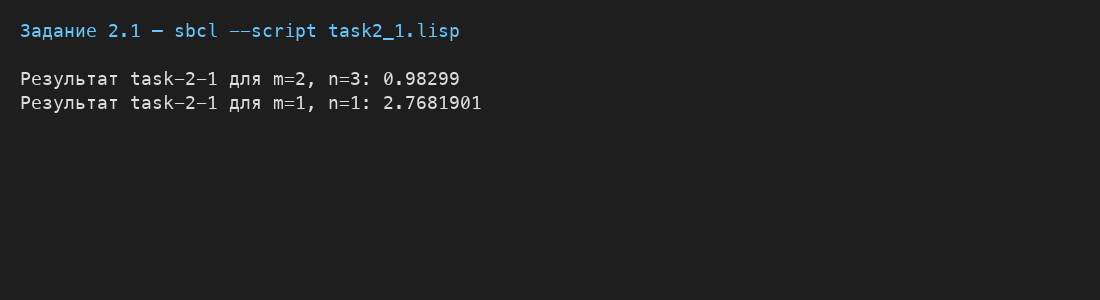
\includegraphics[width=0.85\textwidth]{screenshot_task21.png}
  \caption{Результат выполнения задания 2.1}
  \label{fig:task21}
\end{figure}

\begin{figure}[H]
  \centering
  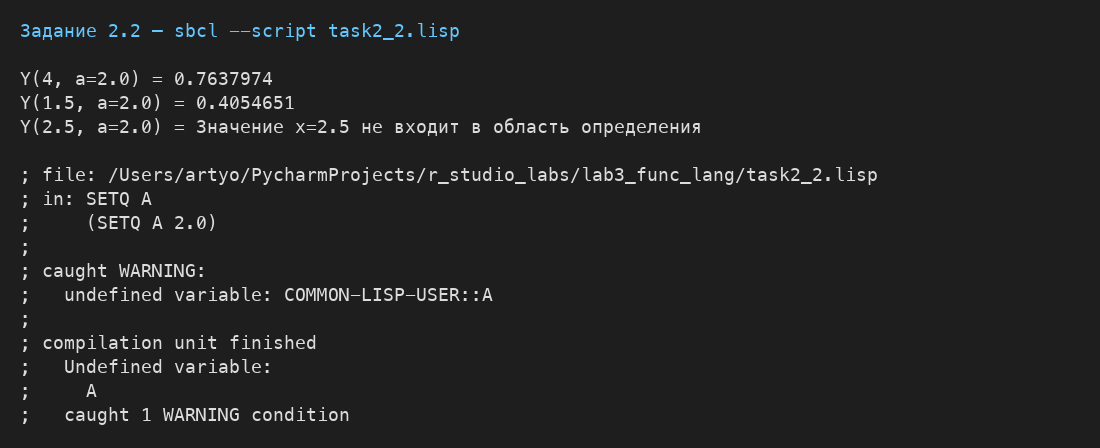
\includegraphics[width=0.85\textwidth]{screenshot_task22.png}
  \caption{Результат выполнения задания 2.2}
  \label{fig:task22}
\end{figure}

\begin{figure}[H]
  \centering
  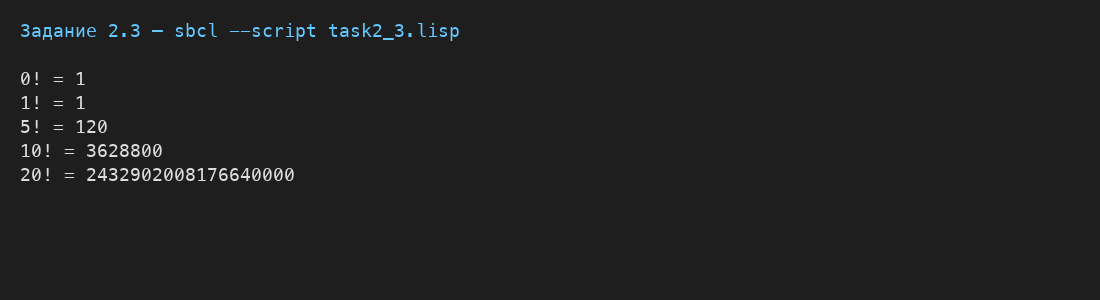
\includegraphics[width=0.85\textwidth]{screenshot_task23.png}
  \caption{Результат выполнения задания 2.3}
  \label{fig:task23}
\end{figure}

\begin{figure}[H]
  \centering
  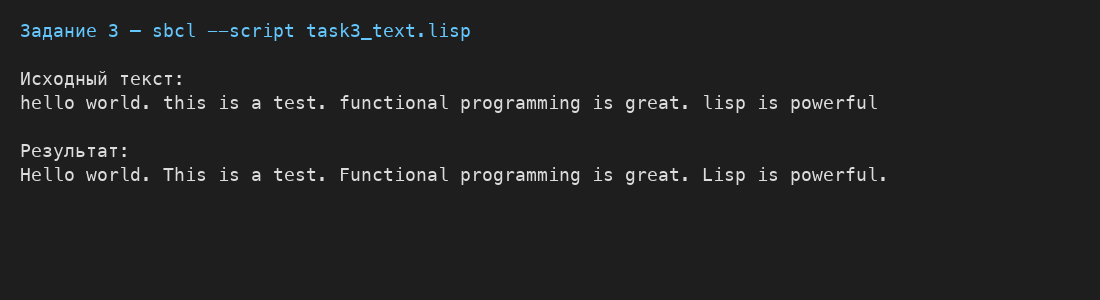
\includegraphics[width=0.85\textwidth]{screenshot_task3.png}
  \caption{Результат выполнения задания 3 (обработка текста)}
  \label{fig:task3}
\end{figure}

\newpage

% =========================================================
% ЗАКЛЮЧЕНИЕ
% =========================================================
\addcontentsline{toc}{section}{Заключение}
\section*{ЗАКЛЮЧЕНИЕ}

В ходе выполнения лабораторной работы были получены следующие результаты:

1 Установлен и настроен интерпретатор SBCL (Steel Bank Common Lisp) и среда разработки Visual Studio Code с расширением Alive для интерактивной работы с Common Lisp.

2 Реализовано вычисление математического выражения варианта~1 с использованием встроенных математических функций Lisp.

3 Реализована функция $Y(x)$ с условным предложением \texttt{COND}, корректно обрабатывающая различные диапазоны входных значений.

4 Реализована рекурсивная функция вычисления факториала с использованием хвостовой рекурсии и аккумулятора.

5 Разработана программа обработки текста на естественном языке с применением функционалов \texttt{mapcar} и \texttt{reduce}, без использования циклов и изменяемых переменных.

6 Изучены основные конструкции языка Common Lisp: определение функций, условные выражения, рекурсия, функции высшего порядка, работа со строками и списками.

\newpage

% =========================================================
% СПИСОК ИСПОЛЬЗОВАННЫХ ИСТОЧНИКОВ
% =========================================================
\addcontentsline{toc}{section}{Список использованных источников}
\section*{СПИСОК ИСПОЛЬЗОВАННЫХ ИСТОЧНИКОВ}

\begin{enumerate}[label=\arabic*,leftmargin=1.25cm]
  \item HomeLisp~-- учебная реализация Лиспа [Электронный ресурс].~-- Режим доступа: \url{https://homelisp.ru/}.~-- Дата доступа: 10.04.2026.
  \item Haskell home page [Электронный ресурс].~-- Режим доступа: \url{https://haskell.org}.~-- Дата доступа: 10.04.2026.
  \item F\# Software Foundation [Электронный ресурс].~-- Режим доступа: \url{https://fsharp.org}.~-- Дата доступа: 10.04.2026.
  \item Официальный сайт Clojure [Электронный ресурс].~-- Режим доступа: \url{https://clojure.org}.~-- Дата доступа: 10.04.2026.
  \item Официальный сайт Scala [Электронный ресурс].~-- Режим доступа: \url{https://scala-lang.org}.~-- Дата доступа: 10.04.2026.
  \item Steel Bank Common Lisp~-- SBCL [Электронный ресурс].~-- Режим доступа: \url{http://www.sbcl.org/}.~-- Дата доступа: 02.06.2026.
  \item Alive: Common Lisp extension for VS Code [Электронный ресурс].~-- Режим доступа: \url{https://marketplace.visualstudio.com/items?itemName=rheller.alive}.~-- Дата доступа: 02.06.2026.
  \item Visual Studio Code [Электронный ресурс].~-- Режим доступа: \url{https://code.visualstudio.com/}.~-- Дата доступа: 02.06.2026.
  \item Мерц, Д. Функциональное программирование на Python / Д.~Мерц.~-- М.~: АСТ, 2026.~-- 128~с.
\end{enumerate}

\end{document}
